\documentclass{article}
\usepackage[utf8]{inputenc}
\usepackage{graphicx}
\usepackage{natbib}
\usepackage{hyperref}

\title{Software Maintenance and Evolution \\God Components}
\author{Jeroen G S Overschie \& Konstantina Gkikopouli}
\date{November 2020}

\begin{document}

\maketitle

\section{Introduction}
God Components (or 'God objects') are components in a software system that have accumulated a large bulk of classes and lines of code over time. Such really large, bulky components are hard to maintain and to reason about; they are in fact a software \textit{anti-pattern} \citep{smith2000software}. It is preferred to have smaller, isolated components instead. Although it is a common good practice to build software by creating small building blocks of reusable code and accessing them using a declarative and well-documented API, big code-bases might still suffer from scaling issues.

To prevent God Components in your software, it is at all times important to keep refactoring a code-base at the architecture level. Be wary and suspicious about 'vague' abstractions that seem to want to answer too many questions at once \citep{riel1996object}. God Components might be broken up into separate, independent components that each have their separate function. This makes the code easier to test and reason about - and above all; more understandable to the humans actually maintaining the code-base.

In this project, one such analysis will be ran on the \textbf{Apache Tika} project \citep{apache_software_foundation_2020}. Apache Tika is a software package built to detect and extract text and metadata from many different file formats. File formats include PDF, PPT and XLS, and can all be accessed through Tika's API, making it easy to process a large amount of files using just a concise amount of code. Besides its text extraction capabilities, it is also commonly used to classify documents using meta-data obtain from Tika, such as any file's extension \citep{Tika}.

God Components will not only be identified, but their evolution over time will also be tracked. This will be done by searching for commits associated to one such God Component and observing either growth or shrinkage. Finally, 

\section{Exploration (week 1)}
First, we explore our chosen software project, Apache Tika, by means of \textbf{requirements analysis}. \citep{dresner1964maintenance}. Requirements were compiled using the project's public website \citep{apache_software_foundation_2020} and an online book about Apache Tika written by the authors \citep{tika_in_action}. 

\subsection{Key design goals}
Let us denote the most important goals the authors set out to accomplish in creating Apache Tika.
\subsubsection{Unified parsing}
One of the initial key goals set by the creators of Apache Tika was the implementation of a unified parsing interface.  In Apache Tika, unified parsing offers a collection of functionalities and a Java interface that deal with external third-party parsing libraries. This was achieved by the creation of the org.apache.tika.parser.Parser interface, which parses the received content incrementally.

\subsubsection{Low Memory Footprint and Fast Processing}
The second goal of the authors regarding Apache Tika was to achieve a low memory footprint and guarantee a fast processing performance. The creators wanted to make sure that Tika could be easily integrated into any Java application at a low memory cost. This would be beneficial to the users, as they could run Tika in any environment ranging from mobile PDA to desktop computers. At the same time, Tika is expected to react quickly to user’s requests and perform file format identification and processing in a fast manner.

As mentioned previously, the received content is parsed incrementally and it is generated as SAX-based XHTML events. SAX (Simple API for XML processing) was the main XML parsing option, as it accomplished all the requirements regarding low memory footprint, fast processing and incremental parsing. In addition, SAX model is more flexible, as it allows its users to decide themselves on how they want to deal with the received content by modifying Tika’s parser and specifying what needs to be done atorg.xml.sax.ContentHandlers.

\subsubsection{Flexible Metadata}
Another design consideration was to ensure the required flexibility that Tika needs in order to perform its tasks on the extracted content. There is an enormous amount of available file formats and Tika is capable of understanding and processing all of them. However, most of these formats contain associated metadata models that provide detailed descriptions about these files. In this case, Tika should also be able to understand the corresponding metadata models. In the previous releases, Tika was always modifying and generalizing the metadata of the extracted content, so that it could fit to its predefined structure. In the latest releases, Tika is not following the same technique and it has become more flexible, as it stores the metadata in their original form.

\subsubsection{Parser integration}
Another key design goal that was taken into account was the parser integration. Similar to the metadata models and file formats, there are also a lot of parsing libraries and Tika has to easily integrate them within the application. According to the creators, from a design perspective Tika virtualizes the underlying parser libraries and ensures their conformance to Tika’s parser interface. However, this is a complicated task as the authors had to deal with parser exceptions, threads of control, delegation, and nuances in each of these libraries. Even though it was a cost-effective process, it brought a lot of benefits like cross-document comparison, uniformity, standardized metadata and extracted text.

\subsubsection{MIME Database}
Another design consideration was focused on the usage of MIME database, which contains a simple and an efficient way of categorizing the file formats. The main goal of the authors was for Tika to support a flexible mechanism that could in a user-friendly way define and identify different media types. Moreover, Tika contains an XML-based mechanism that is responsible for adding new media types, regular expressions and glob patterns.

\subsubsection{MIME Detection}
Based on the previous section, the authors continued with making different flexible MIME detection tools available to the end users, like via byte[] arrays, java.io.Files, filenames and java.net.URLs pointing to the files etc. They  also focused on making the MIME information available to Tika’s parser and metadata, because the detected media type could be an essential source of information to return as extracted metadata along with the parsing operation.

\subsubsection{Language detection}
Language detection has also become an important feature in Tika. The ability of understanding a language is essential, as it provides useful information regarding the content of the file and its corresponding metadata. Nowadays, the developers are trying to improve language detection in Tika by adding tools that improve language-specific charset detection in the parser.

\subsection{Quality attributes}
\begin{enumerate}
    \item Reliability. In order for any professional to be able to use Tika in a production environment, the program must be reliable and produce consistent results.
    \item Usability. The program should be usable both in terms of User Experience (UX) and programming interface (API); this means it should have a nice and well-functioning GUI and CLI to use the program and an API to use Tika in your own program code.
    
    \begin{quote}
        ``By adopting the SAX model, Tika allows developers and those wishing to customize how Tika’s Parser deals with extracted information to define..."
    \end{quote}
    
    \begin{quote}
        ``The Tika facade (center of the diagram) is a simple, easy-to-use frontend to all of Tika’s capabilities..."
    \end{quote}
    
    
    \begin{quote}
        ``Tika should be embeddable within Java applications at low memory cost so that it’s as easy to use Tika in a desktop-class environment with capacious network..."
    \end{quote}
    
    \item Correctness. It is important the program produces correct results, i.e. outputs corrects meta data about files. In the case of too many errors, developer trust will dissipate.
    \item Flexibility. Flexibility is a significant requirement and it is quite emphasized on Tika's documentation. In general, flexibility represents the capability of a given system to adapt to different environments, settings or to adjust when changes occur.
    
    \begin{quote}
        ``First and foremost, we wanted Tika to support a flexible mechanism to define media types..."
    \end{quote}
    
    \begin{quote}
        ``By adopting the SAX model, Tika allows developers and those wishing to customize how Tika’s Parser deals with extracted information to define custom parsers..."
    \end{quote}
    
    \begin{quote}
        ``Provide Flexible MIME Detection:To expose the MIME information programmatically, we decided to expose as many MIME detection mechanisms..."
    \end{quote}
    
    \begin{quote}
        ``Beyond that detail (Tika opted to allow one to many types per Parser, achieving the greatest flexibility and decreasing the overall number of parsers), the exchange of MIME information between Parser and Metadata object was another important consideration..."
    \end{quote}
    \item Performance. Performance is also another significant requirement in Tika. It demonstrates how the systems reacts while performing given tasks at a certain time. The creators of Tika developed Tika in a way that it could respond fast to requests. Although at the time of its making not similar products might have existed, Tika would have been quickly superseded if it was not performing well enough. So in order to be able to process large datasets the program has to be of sufficient speed.
    
    \begin{quote}
        ``The necessity of detecting file formats and understanding them is pervasive within software, and thus we expect Tika to be called all the time, so it should respond quickly when called upon.."
    \end{quote}
    
    \begin{quote}
        ``SAX, on the other hand, parses tags incrementally, causing a low memory footprint, allowing for rapid processing times..."     \end{quote}
    
    \item Integrability. In general terms, integrability shows the capability of a system to integrate with other components or systems. 
    
    \begin{quote}
        ``External interfaces, including the command line and a graphical user interface allow users to integrate Tika into their scripts and applications and to interact with Tika visually."
    \end{quote}
    
    \begin{quote}
        ``Parser integration: Just as there are many metadata models per file format, there are also many parsing libraries. Tika should make it easy to use these within an application."
    \end{quote}
    
\end{enumerate}

% \textbf{Functional requirements:}
% \begin{itemize}
%     \item Extract file meta-data
%     \begin{itemize}
%         \item File extension
%         \item File size
%         \item Last-modified
%         \item ...
%     \end{itemize}
%     \item Extract file text
%     \item Well-documented API to pragmatically interact with the program
%     \item Command-line interface to interactively interact with the program
% \end{itemize}

% \textbf{Non-functional requirements:}
% \begin{itemize}
%     \item GUI to use program capabilities for non-programmers
%     \item REST API for submitting extraction tasks
%     \item Text translation using Microsoft Translation API
%     \item Text language identification 
%     \item Stream analysed plain-text in chunks
%     \item Extract phone numbers
% \end{itemize}

\section{System structure (week 2)}
An analysis will be performed using common Software Engineering tooling programs. We first ran the program byte-code through \textit{Structure101}, see Figure~\ref{fig:structure101}.

\begin{figure}
    \centering
    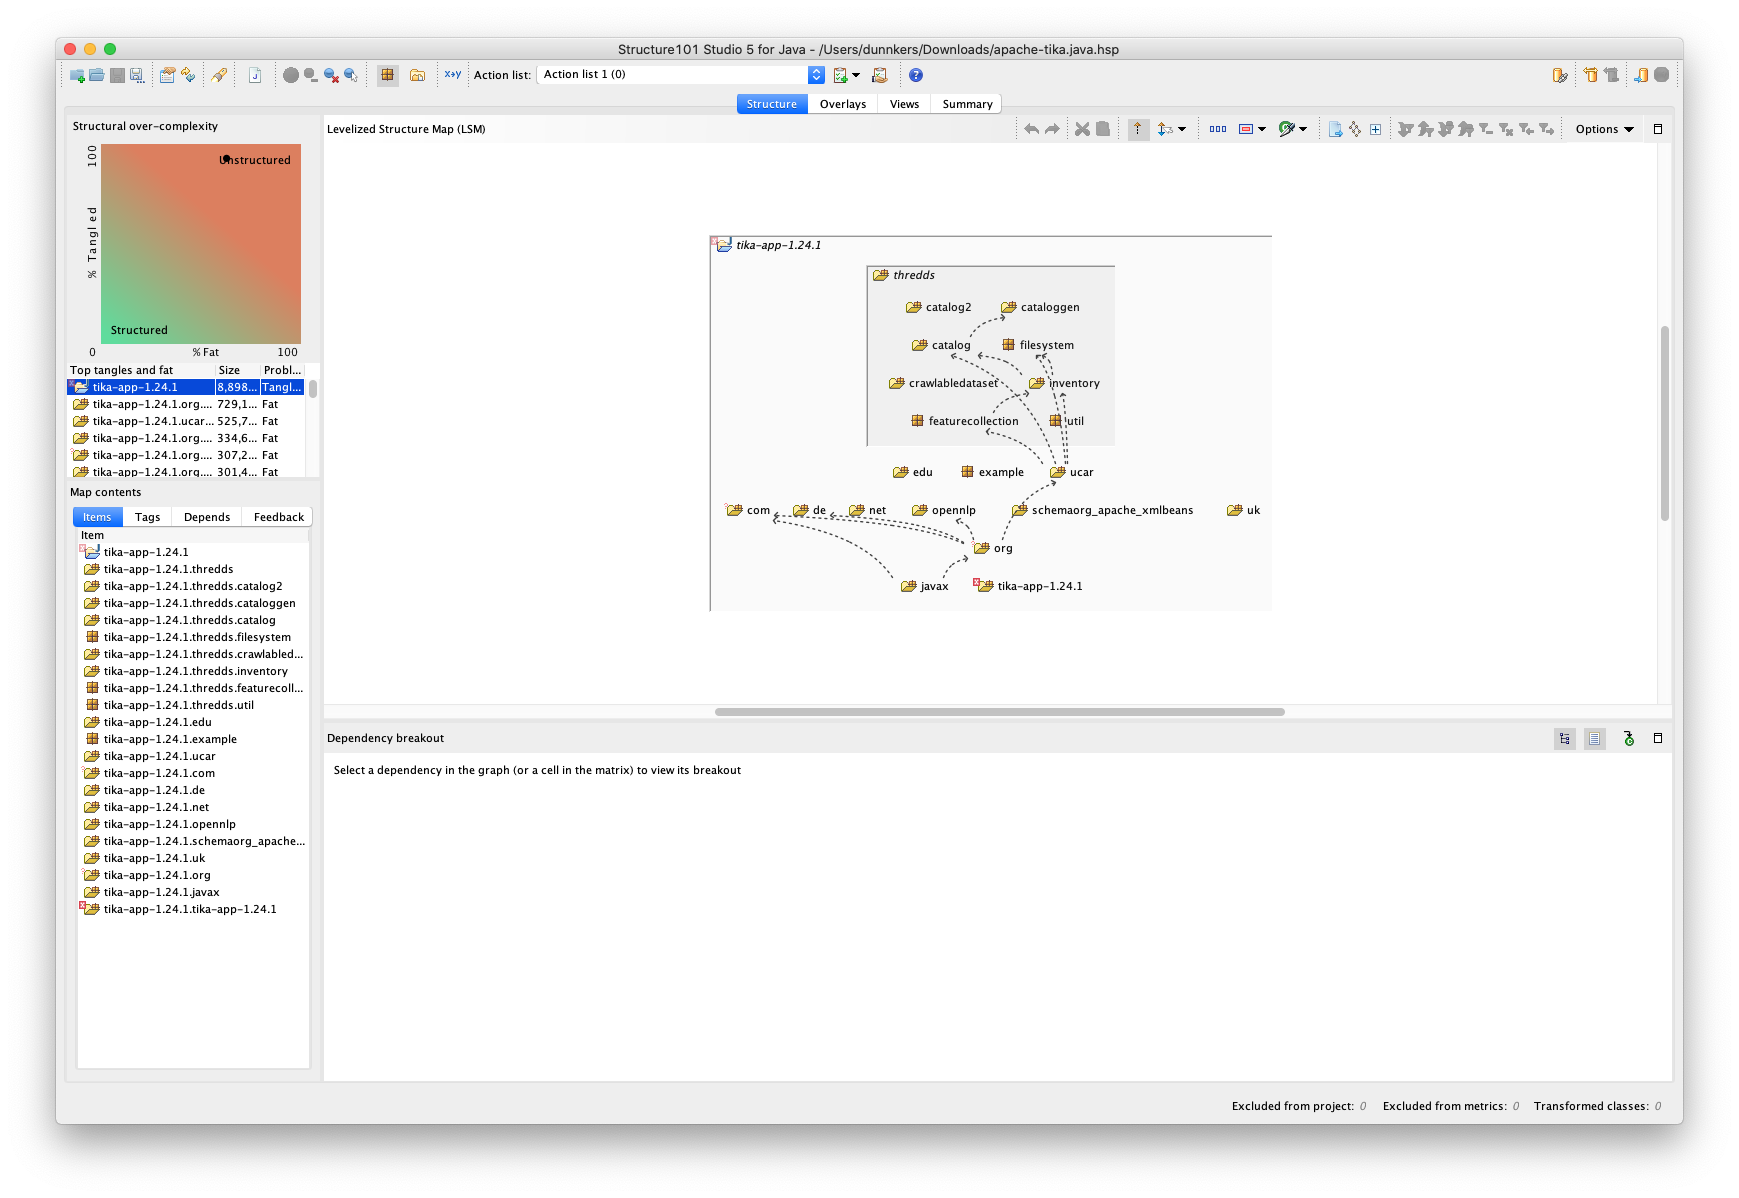
\includegraphics[width=\textwidth]{structure101.png}
    \caption{Structure101 overview of Apache Tika.}
    \label{fig:structure101}
\end{figure}

% \section{Identifying God Components (week 3 and 4)}
% identify god components using (1) our own code (2) Designite

% - find commits linked to: adding- or removing code to god components

% - create timeline for god components evolution

\bibliographystyle{plain} % We choose the "plain" reference style
\bibliography{bibliography}

\end{document}
